\section{Grundlagen}
\subsection{Vierpoldarstellung}
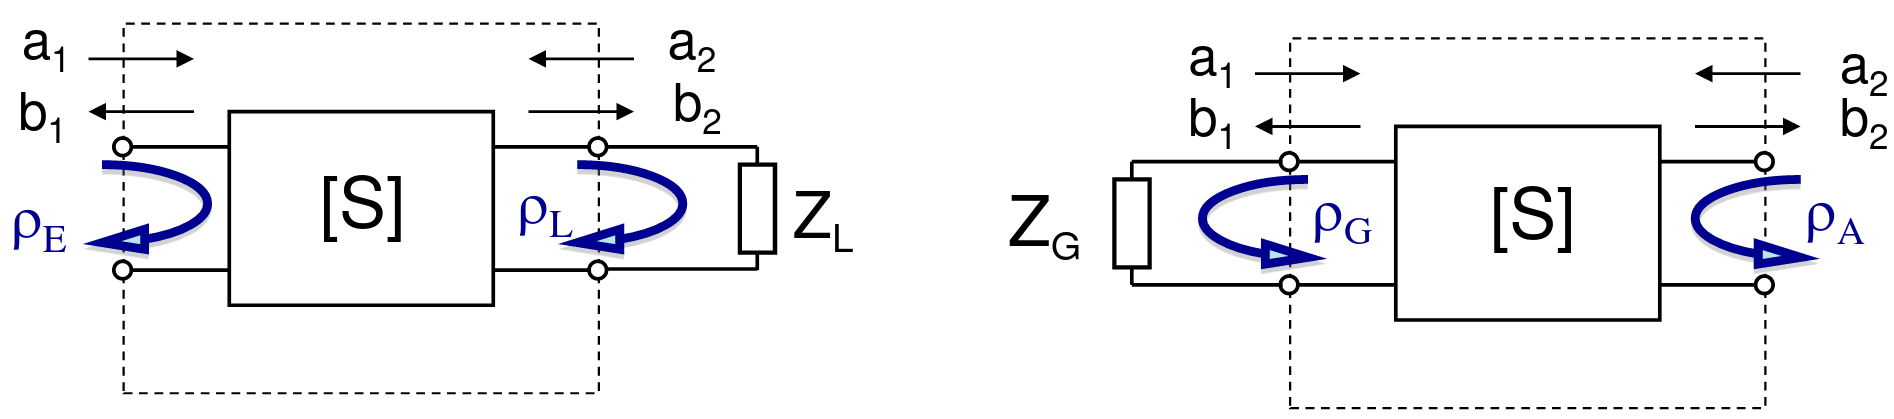
\includegraphics[width=0.35\paperheight]{content/hfmess/pictures/hf_zweitor_reflektion.png}
\begin{itemize}
    \itemsep0pt
    \item \textbf{Anpassung:} allseits reflexionsfrei\\
        \(s_{ii} = 0, \;\forall i \in (1;\; \mathrm{dim}(S))\)
    \item \textbf{Reziprozität} (Übertragungssymmetrie): \(S = S^\top\)
    \item \textbf{Verlustfreie} n-Tore ($S$ unitär):\\
        \(\sum^n_{i=1} |b_i|^2 = \sum^n_{i=1} |a_i|^2 \implies S^\top S^* = I\)
    \item \textit{Allgemein:} \(\underline{b} = S \underline{a}\)
    \item Reflexion $\leftrightarrow$ Impedanz:\\
    \(\rho = \dfrac{z-1}{z+1},\;\; z = \dfrac{\rho+1}{\rho-1},\;\; z=\dfrac{Z}{Z_0}\)
   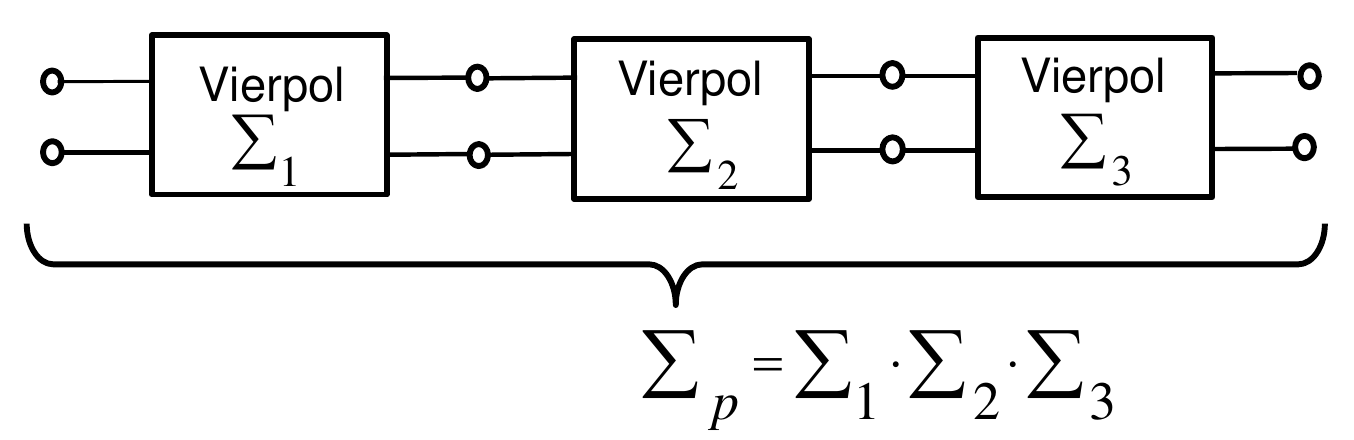
\includegraphics[width=0.35\paperheight]{content/hfmess/pictures/transmissionsmatrix.png}
    \item Beschreibungsformen eines \textbf{HF-Zweitors}:
    \begin{align*}
        \parbox{2cm}{Streumatrix:}
        \begin{bmatrix}\
            b_1\\
            b_1\
        \end{bmatrix}\
        &=\
        \begin{bmatrix}\
            S_{11} & S_{12}\\
            S_{21} & S_{22}\
        \end{bmatrix}\
        \begin{bmatrix}\
            a_1\\
            a_2\
        \end{bmatrix}\\
        \parbox{2cm}{Wellentrans- missionsmatrix:}
        \begin{bmatrix}\
            b_1\\
            a_1\
        \end{bmatrix}\
        &=\
        \begin{bmatrix}\
            \Sigma_{11} & \Sigma_{12}\\
            \Sigma_{21} & \Sigma_{22}\
        \end{bmatrix}\
        \begin{bmatrix}\
            a_2\\
            b_2\
        \end{bmatrix}\\
        \parbox{2cm}{ABCD-Matrix:}
        \begin{bmatrix}\
            u_1\\
            i_1\
        \end{bmatrix}\
        &=\
        \begin{bmatrix}\
            A & B\\
            C & D\
        \end{bmatrix}\
        \begin{bmatrix}\
            u_2\\
            -i_2\
        \end{bmatrix}\\
    \end{align*}
    \item $u$ und $i$ sind normierte Spannungen und Ströme (Einheit: Qudratwurzel der Leistung):
    \begin{equation*}
        u = \dfrac{U}{\sqrt{Z_0}},\;\; i = I \sqrt{Z_0}
    \end{equation*}
    \item Umrechnung Streumatrix $\leftrightarrow$ Transmissionsmatrix:
        \begin{align*}
            [\Sigma]\
            &=\
            \dfrac{1}{S_{21}}\
            \begin{bmatrix}\
                    -\Delta_S & S_{11}\\
                    -S_{22} & 1\
            \end{bmatrix}\\
            [S]\
            &=\
             \dfrac{1}{\Sigma_{22}}\
            \begin{bmatrix}\
                    \Sigma_{12} & -\Delta_\Sigma\\
                    1 & -\Sigma_{21}
            \end{bmatrix}\\
            \Delta_S &= S_{11}S_{22} - S_{12}S_{21},\\
            \Delta_\Sigma &= \Sigma_{11}\Sigma_{22} - \Sigma_{12}\Sigma_{21}
        \end{align*}
        \item Umrechnung ABCD $\leftrightarrow$ Streumatrix:
            \begin{align*}
                S_{11} &= \dfrac{A+B-C-D}{A+B+C+D}, &S_{12} = \dfrac{2\:\Delta_{\mathrm{ABCD}}}{A+B+C+D},\\
                S_{21} &= \dfrac{2}{A+B+C+D}, &S_{22} = \dfrac{-A+B-C+D}{A+B+C+D},\\\\
                A &= \dfrac{-\Delta_S + S_{11} - S_{22} + 1}{2 S_{21}},
                &B = \dfrac{\Delta_S + S_{11} + S_{22} + 1}{2 S_{21}},\\
                C &= \dfrac{\Delta_S - S_{11} - S_{22} + 1}{2 S_{21}},
                &D = \dfrac{-\Delta_S - S_{11} S_{22} + 1}{2 S_{21}}
            \end{align*}
        \item Längwiderstand bzw. Querleitwert mit Bezugswiderstand $Z_0$:\\
            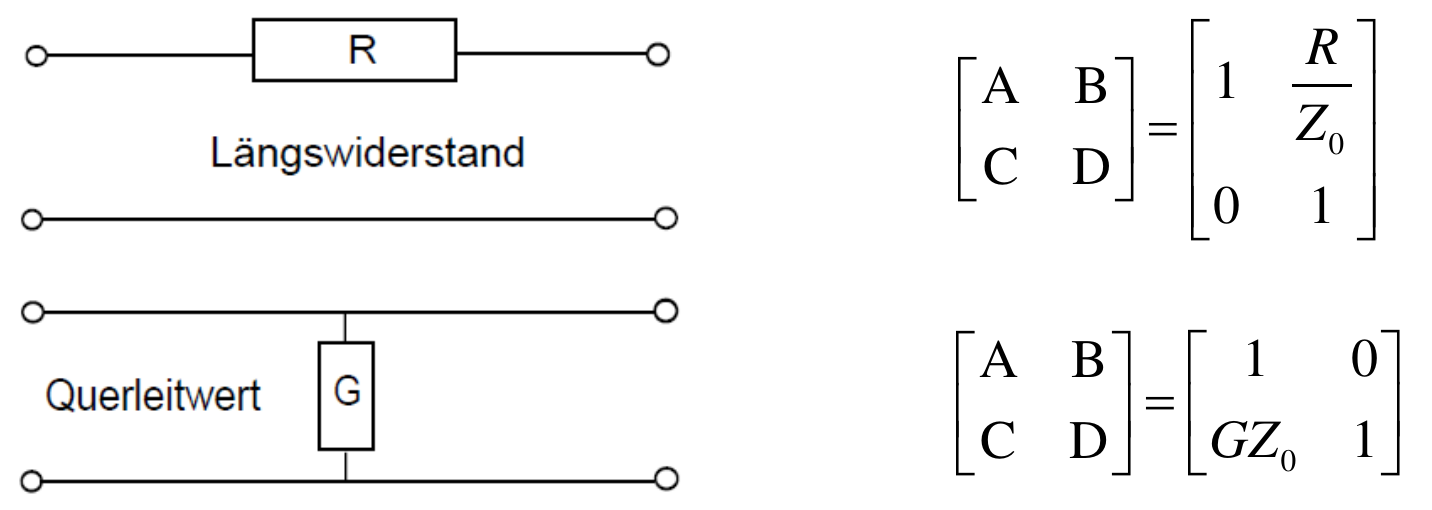
\includegraphics[width=0.35\paperheight]{content/hfmess/pictures/kettenmatrix_widerstand_leitwert.png}
        \item Verlustlose Leitung (Wellenwiderstand $Z_l$, elektrische Länge $\beta l$, geometrische Länge $l$):
        \begin{align*}
            &\parbox{2.5cm}{Verlust\textit{lose} Leitung:}
            \begin{bmatrix}\
                A & B\\
                C & D\
            \end{bmatrix}\
            &=\
            \begin{bmatrix}
                \cos\beta l & j\frac{Z_1}{Z_0}\sin\beta l\\
                j\frac{Z_0}{Z_1}\sin\beta l & \cos \beta l\
            \end{bmatrix}\\
            &\parbox{2.5cm}{Verlustbehaftete Leitung:}
            \begin{bmatrix}\
                A & B\\ C & D\
            \end{bmatrix}\
            &=\
            \begin{bmatrix}
                \cosh\gamma l & j\frac{Z_1}{Z_0}\sinh\gamma l\\
                j\frac{Z_0}{Z_1}\sinh\gamma l & \cosh\gamma l\
            \end{bmatrix}\\
            &\parbox{2.5cm}{Verlustloser Übertrager:}
            \begin{bmatrix}\
                A & B\\
                C & D\
            \end{bmatrix}\
            &=\
            \begin{bmatrix}
                \frac{1}{n} & 0\\
                0 & n\
            \end{bmatrix}
        \end{align*}
        \begin{align*}
            &Z_1: \text{(kompl.) Wellenwiderstand,}\\
            &\beta l: \text{elek. Länge,}\\
            &l: \text{geom. Länge,}\\
            &\gamma: \text{kompl. Ausbreitungskonstante,}\\
            &n: \text{Windungsverhältnis } N_1/N_2
        \end{align*}
\end{itemize}


